\chapter{Lezione 4}
\label{chap:lezione_04} 

\begin{flushright}
\textit{Data: 09/10/2025}
\end{flushright}


\section{Estensione del Teorema Centrale del Limite per code pesanti }

L'analisi dei momenti di una distribuzione a legge di potenza ($\rho(x) \sim x^{-\alpha}$) è fondamentale per comprendere il comportamento del Teorema Centrale del Limite.

Ricordiamo le condizioni di finitudine per i momenti:
\begin{itemize}
    \item La media $\langle x \rangle$ è finita per $\alpha > 2$.
    \item La varianza $\langle x^2 \rangle$ è finita per $\alpha > 3$.
\end{itemize}

L'obiettivo è estendere l'equazione del TLC a diversi casi. Iniziamo considerando il caso in cui $\alpha > 3$, ovvero la varianza è finita.

\subsection{Calcolo del Terzo Cumulante}

Per il caso in cui $\langle x^2 \rangle$ è finito, consideriamo momenti di ordine superiore (cumulanti di ordine $m \ge 3$) e consideriamo $\alpha$ appena superiore a 3, definendo:

\begin{equation}
\alpha = 3 + \delta
\end{equation}

dove $\delta > 0$.

Per una variabile casuale gaussiana, tutti i cumulanti di ordine $m \ge 3$ sono nulli, e la distribuzione della somma di variabili IID (Indipendenti e Identicamente Distribuite) converge a una Gaussiana. Vogliamo verificare se questo accade anche in questo caso, calcolando il terzo cumulante $C_{3,1}$ per una singola variabile.

Il cumulante di ordine tre per una singola variabile è dato dall'integrale, dove $X_N$ è il valore massimo delle $N$ estrazioni:

\begin{equation}
C_{3,1}\sim\int_{m}^{x_{N}}dx(\alpha-1)m^{\alpha-1}x^{-\alpha}(x-\mu)^{3}
\end{equation}

Espandendo l'integrale (utilizzando i termini dominanti della PDF come $\rho(x) \sim x^{-\alpha}$ e $\rho(x) (x-\mu)^3 \sim x^{3-\alpha}$):

\begin{equation}
=\int_{m}^{x_{N}}dx \; (x^{3-\alpha}-x^{-\alpha}\mu^{3}-3x^{2-\alpha}\mu-3x^{1-\alpha}\mu^{2}) 
\end{equation}

Sostituendo $\alpha = 3 + \delta$:

\begin{equation}
=\int_{m}^{x_{N}}dx(x^{-\delta}-x^{-3-\delta}\mu^{3}-3x^{-1-\delta}\mu-3x^{-2-\delta}\mu^{2}) 
\end{equation}

Il termine dominante nell'integrale è $x^{-\delta}$. L'integrazione fornisce:

\begin{equation}
C_{3,1}\sim\int_{m}^{x_{N}}x^{-\delta}dx\sim x_{N}^{1-\delta}-m^{1-\delta}
\end{equation}

Il termine dominante dipende dal valore di $\delta$:
\begin{itemize}
    \item Se $\delta > 1$ (ovvero $\alpha > 4$), l'esponente $1-\delta$ è negativo. Per $X_N \to \infty$, il termine $X_N^{1-\delta}$ tende a zero, e $C_{3,1}$ è una costante. Questo caso non è molto interessante.
    \item Se $0 < \delta < 1$ (ovvero $3 < \alpha < 4$), l'esponente $1-\delta$ è positivo e il termine dominante è $X_N^{1-\delta}$. Poiché $X_N \sim N^{1/(\alpha-1)} = N^{1/(2+\delta)}$, si ha:
    \begin{equation}
    C_{3,1}\sim N^{\frac{1-\delta}{2+\delta}}
    \end{equation}
\end{itemize}

\subsection{Cumulanti della Variabile Scalata }

Definiamo la variabile scalata $V$ (standardizzata) per la somma $Y = \frac{1}{N}\sum_i x_i$:

\begin{equation}
V:v=(Y-\mu_{0})\frac{\sqrt{N}}{\sigma_{0}}
\end{equation}

Per questa variabile standardizzata, i cumulanti di una Gaussiana sono $C_{1,v}=0$ e $C_{2,v}=1$. Vogliamo verificare la tendenza a zero dei cumulanti di ordine superiore, come $C_{3,v}$.

Il cumulante $C_{m}$ della media di $N$ variabili $\bar{X}$ è legato al cumulante della singola variabile $C_{m,1}$ dalla relazione:

\begin{equation}
C_{m, \bar{X}} = \frac{C_{m,N}}{N^{m}} = \frac{1}{N^{m}} C_{m,1} N = C_{m,1} N^{1-m}
\end{equation}

Il cumulante $C_{m,v}$ per la variabile scalata $V$ (normalizzata per deviazione standard) è dato da:

\begin{equation}
C_{m, v}=\frac{C_{m, 1}}{\sigma_{0}^{m}}N^{1-m/2}
\end{equation}

Per $m=3$, il terzo cumulante scalato è:

\begin{equation}
C_{3,v}=\frac{C_{3,1}}{\sqrt{N}{\sigma_{0}}^{3}}
\end{equation}

Sostituendo la dipendenza da $N$ di $C_{3,1}$ per $3 < \alpha < 4$:

\begin{equation}
C_{3,\nu}\sim N^{\frac{1-\delta}{2+\delta}}N^{-1/2}\sim N^{-\frac{3\delta}{2(2+\delta)}}
\end{equation}

Poiché $\delta > 0$, l'esponente è negativo. Quindi, per $N \rightarrow \infty$, si ha $C_{3,v} \rightarrow 0$.

In generale, il cumulante di ordine $m$ per la singola variabile scala come:
\begin{equation}
C_{m,1}\sim N^{\frac{m-2-\delta}{2+\delta}}
\end{equation}

E il cumulante di ordine $m$ per la variabile scalata $V$ scala come:
\begin{equation}
C_{m, v}\sim N^{\frac{-m\delta}{2(2+\delta)}} \rightarrow 0 \quad \text{per } N\rightarrow\infty
\end{equation}

Nel caso in cui $\alpha > 3$ (varianza finita), tutti i cumulanti di ordine $m \ge 3$ della variabile scalata $V$ tendono a zero. La distribuzione limite è dunque la \textbf{Distribuzione Gaussiana}. Per $\alpha > 3$ , dunque, una power law segue il Teorema Centrale del Limite.

\section{Distribuzioni Stabili di Lévy per code molto pesanti }

Consideriamo ora il caso in cui $1 < \alpha < 3$, dove la varianza è divergente. Il TLC non si applica, ma la distribuzione limite della somma di variabili converge a una \textbf{Distribuzione Stabile di Lévy}.

\subsection{La Funzione Caratteristica $\hat{\rho}(z)$}

La distribuzione di probabilità $\rho(x)$ per una variabile simmetrica con legge di potenza nelle code è:
\begin{equation}
\rho(x)=\begin{cases}\frac{1}{2}(\alpha-1)m^{\alpha-1}|x|^{-\alpha} & |x|\ge m \\ 0 & |x|<m\end{cases}
\end{equation}

\begin{figure}[h]
    \centering
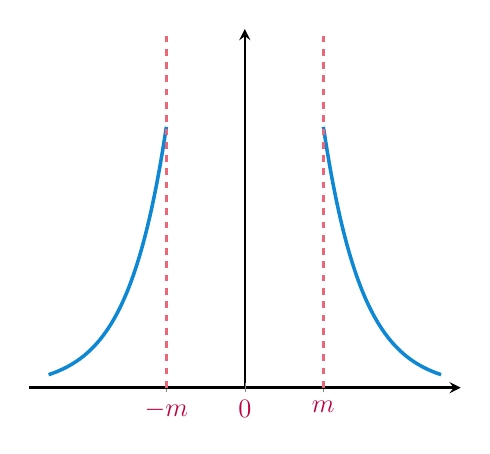
\begin{tikzpicture}[scale=0.8]
    \begin{axis}[
        axis lines = middle,
        xmin = -5.5, xmax = 5.5,
        ymin = 0, ymax = 5.5,
        xtick = {-2, 2},
        xticklabels = {$-m$, $m$},
        ytick = \empty,
        extra x ticks = {0},
        extra x tick labels = {0},
        thick,
        xlabel = {}, ylabel = {},
        tick label style = {font=\large, color=purple},
        axis line style = {very thick}
    ]

    % Parametro m (distanza dall'asse y)
    \def\m{2}

    % Parte sinistra del grafico (fino a -m)
    \addplot [
        domain=-5:-2, 
        samples=100, 
        color=cyan!70!blue, 
        ultra thick
    ] {exp(x+2) * 4};

    % Parte destra del grafico (da m in poi)
    \addplot [
        domain=2:5, 
        samples=100, 
        color=cyan!70!blue, 
        ultra thick
    ] {exp(-x+2) * 4};

    % Linee tratteggiate verticali rosa
    \draw [dashed, ultra thick, red!50!purple!60] (axis cs:-2,0) -- (axis cs:-2,5.5);
    \draw [dashed, ultra thick, red!50!purple!60] (axis cs:2,0) -- (axis cs:2,5.5);

    \end{axis}
\end{tikzpicture}
\caption{Distribuzione di probabilità $\rho(x)$.}
\end{figure}

La funzione caratteristica $\hat{\rho}(z)$ è calcolata come:
\begin{equation}
1-\hat{\rho}(z)=\int_{-\infty}^{-m}dx \; (1-e^{izx})\rho(x)+\int_{m}^{\infty}dx~\rho(x)(1-e^{izx})
\end{equation}
\begin{equation}
=\left [\frac{(\alpha-1)m^{\alpha-1}}{2}\right ] \left [\int_{-\infty}^{-m}(-x)^{-\alpha}(1-e^{izx})dx+\int_{m}^{\infty}dx~x^{-\alpha}(1-e^{izx})\right ] 
\end{equation}
\begin{equation}
=\left [\frac{(\alpha-1)m^{\alpha-1}}{2}\right ] \left [\int_{m}^{\infty}dx~x^{-\alpha}(1-e^{-izx})+\int_{m}^{\infty}dx~x^{-\alpha}(1-e^{izx})\right ] 
\end{equation}

Dopo un cambio di variabile $u=|z|x$, si ottiene l'approssimazione:
\begin{equation}
1-\hat{\rho}(z)=1-(\alpha-1)(m|z|)^{\alpha-1}\int_{m|z|}^{+\infty}du \; \frac{1-\cos u}{u^{\alpha}}
\end{equation}

Per $u<<1$ vale: $1-\cos u \approx \frac{u^2}{2}$ 

Segue:
\begin{equation}
\int_{m|z|}^{+\infty}du \; u^{2-\alpha} \approx |z|^{3-\alpha}
\end{equation}

per $\alpha >3$ diverge, ma stiamo considerando il caso $1 < \alpha < 3$

Per $|z|<<1$ si ha:

\begin{equation}
\hat{\rho}(z)=1-K|z|^{\alpha-1}
\end{equation}
dove $K$ è una costante definita come:
\begin{equation}
K=(\alpha-1)m^{\alpha-1}C
\end{equation}
con la costante $C$ data da:
\begin{equation}
C=\int_{0}^{\infty}du\frac{1-cosu}{u^{\alpha}}= \alpha \Gamma(\alpha)\sin(\frac{\pi \alpha}{2})
\end{equation}

Questa forma è valida per $1 < \alpha < 3$.

\subsection{Distribuzione Limite}

Per trovare la distribuzione limite della somma di $N$ variabili, si usa un fattore di riscalamento diverso rispetto al TLC, basato sul valore massimo $\max\{x_i\}$ invece che sulla deviazione standard $\sigma_0$. Definiamo la variabile riscalata $V$ come:
\begin{equation}
V:v=\frac{S}{X_{N}}=\frac{\sum_{i}x_{i}}{\max\{x_{i}\}}
\end{equation}
dove $\max\{x_i\} \sim N^{1/(\alpha-1)}$.

La funzione caratteristica della somma riscalata è:
\begin{equation}
\hat{\rho}_{v}(z)=\hat{\rho}(|z|N^{-\frac{1}{\alpha-1}})^{N}\sim(1-K|z|^{\alpha-1}N^{-\frac{\alpha-1}{\alpha-1}})^{N}
\end{equation}

\begin{equation}
\sim(1-\frac{K|z|^{\alpha-1}}{N})^{N}\xrightarrow{N\rightarrow\infty} e^{-K|z|^{\alpha-1}} \quad \quad  \quad  \text{(\textbf{Distribuzione di Lévy})}
\end{equation}

Per $\alpha=2$ (dove la media è finita ma la varianza è infinita), la distribuzione limite è la \textbf{Distribuzione di Cauchy}:
\begin{equation}
\hat{\rho}_{v}\sim e^{-K|z|}\rightarrow\rho_{v}(x)=\frac{1}{\pi}\frac{K}{K^{2}+x^{2}}
\end{equation}

\newpage
\section{Legge di Benford e Processi Moltiplicativi}

La \textbf{Legge di Benford} descrive la probabilità $P(n)$ che la prima cifra significativa di un insieme di numeri sia $n$ (con $n=1, \dots, 9$). A differenza di una distribuzione uniforme ($P(n) \approx 1/9$), la Legge di Benford prevede che le cifre più piccole (soprattutto $n=1$) siano più frequenti.

\begin{figure}[h!]
    \centering
    \begin{tikzpicture}[scale=0.7]
        \begin{axis}[
            width=12cm,
            height=8cm,
            title={First 100.000 Fibonacci Numbers},
            xlabel={First Digit},
            ylabel={Probability},
            ymin=0, ymax=0.32,
            xmin=0.5, xmax=9.5,
            xtick={1,2,3,4,5,6,7,8,9},
            ytick={0, 0.05, 0.10, 0.15, 0.20, 0.25, 0.30},
            ymajorgrids=false,
            axis line style={gray!50},
            tick label style={font=\small, /pgf/number format/fixed, /pgf/number format/precision=2},
            legend style={at={(0.95,0.8)}, anchor=north east, draw=none, fill=none, font=\small},
            bar width=1.0, % Per rendere le barre adiacenti come nell'originale
        ]

        % Istogramma (Distribuzione delle prime cifre dei numeri di Fibonacci)
        % Valori approssimati basati sulla legge di Benford (a cui i Fibonacci convergono)
        \addplot[
            ybar,
            fill=colorD!50,
            draw=white,
            area legend
        ] coordinates {
            (1, 0.301) (2, 0.176) (3, 0.125) (4, 0.097) (5, 0.079) 
            (6, 0.067) (7, 0.058) (8, 0.051) (9, 0.046)
        };
        \addlegendentry{1st digit distribution}

        % Curva di Benford (Tratteggiata)
        \addplot[
            black,
            dashed,
            very thick,
            domain=1:9,
            samples=100,
        ] {log10(1 + 1/x)};
        \addlegendentry{Benford's law}

        \end{axis}
    \end{tikzpicture}
    \caption{Distribuzione della prima cifra per i primi 100.000 numeri della successione di Fibonacci confrontata con la Legge di Benford.}
\end{figure}

\subsubsection{Derivazione della Legge di Benford}

La probabilità $P(n)$ è definita come la probabilità che un numero $M$ rientri nell'intervallo $\left [n \cdot 10^k, (n+1) \cdot 10^k\right ] $ per qualsiasi scala $k$:

\begin{equation}
P(n) = \sum_{k} \int_{n \cdot 10^{k}}^{(n+1) \cdot 10^{k}} \rho(M) dM
\end{equation}

Questa formulazione approssimativa somma tutte le possibili scale $k$.

Il secondo punto fondamentale è l' \textbf{Invarianza di Scala}. Se si cambia l'unità di misura (la scala) da $M$ a $bM$ (ad esempio, lunghezza di un fiume in km o cm), la distribuzione di probabilità $\rho(M)$ non deve cambiare.
L'unica distribuzione di probabilità che soddisfa tale relazione di scaling è la legge di potenza $\rho(M) \propto 1/M$.

Sostituendo $\rho(M) \sim 1/M$ nell'integrale, si ottiene:
\begin{equation}
P(n) = \sum_{k} \int_{n \cdot 10^{k}}^{(n+1) \cdot 10^{k}} dM \frac{1}{M} = \sum_{k} \{\log\left [ (n+1)10^{k}\right ]  - \log\left [n10^{k}\right ] \}
\end{equation}
\begin{equation}
P(n) = \sum_{k} \log \frac{n+1}{n}
\end{equation}

Dopo la normalizzazione, la Legge di Benford è data da:
\begin{equation}
P(n) = \log_{10}\left(\frac{n+1}{n}\right)
\end{equation}


\subsubsection{Processo Additivo}

Un processo additivo è definito come una passeggiata aleatoria in cui si aggiunge un termine casuale $\xi$ ad ogni passo temporale $t$:
\begin{equation}
N_{t+1} = N_t + \xi
\end{equation}

Per $\xi$ distribuito simmetricamente con varianza finita, $N_t$ è la somma di $t$ variabili casuali.
La varianza $\sigma^2$ scala linearmente con $t$ e la deviazione standard scala come $\sigma \sim \sqrt{t}$.
Per $t \to \infty$, la distribuzione di $N_t$ diventa sempre più larga e tende a una distribuzione uniforme (che non è una distribuzione di scala).

\subsubsection{Processo Moltiplicativo}

Un processo moltiplicativo (tipico di crescita di popolazioni o variazioni percentuali del mercato azionario) è definito da:
\begin{equation}
N_{t+1} = N_t \cdot \xi
\end{equation}

Prendendo il logaritmo, il processo moltiplicativo si trasforma in un processo additivo nello spazio logaritmico:
\begin{equation}
\log(N_{t+1}) = \log(N_t) + \log(\xi)
\end{equation}

Per $t \to \infty$, il Teorema Centrale del Limite si applica a $\log(N_t)$, e la sua distribuzione converge a una Gaussiana. La distribuzione di $\log(N_t)$ diventa uniforme nello spazio logaritmico.

Una distribuzione uniforme su $\log(N)$ implica $\int p(\log N) d \log N \sim \int \frac{dN}{N}$, ovvero la distribuzione nello spazio lineare è $\rho(N) \propto 1/N$.

La dipendenza da $\frac{1}{N}$ è una caratteristica fondamentale delle distribuzioni che seguono la legge di Benford.

\subsection{La Distribuzione Log-Normale}

Quando una variabile casuale $X$ è il risultato del prodotto di un gran numero $N$ di variabili casuali indipendenti $y_i$:
$$X = \prod_{i=1}^{N} y_i$$

il suo logaritmo sarà la somma di molte variabili casuali:
$$\log X = \sum_{i=1}^{N} \log(y_i)$$

Se le variabili $\log(y_i)$ hanno media $\mu_l$ e varianza $\sigma_l^2$ finite, allora la distribuzione di $\log X$ tenderà a una distribuzione normale (Gaussiana) con media $N\mu_l$ e varianza $N\sigma_l^2$.
$$\tilde{\rho}(\log X) = C \exp\left\{-\frac{(\log X - N\mu_l)^2}{2\sigma_l^2 N}\right\}$$

Di conseguenza, la variabile $X$ segue una \textbf{distribuzione log-normale}. La sua funzione di densità di probabilità $\rho(X)$ si ottiene dalla densità del suo logaritmo $\tilde{\rho}(\log X)$ con un cambio di variabile:
$$\rho(X)dX = \tilde{\rho}(\log X) d\log X = \tilde{\rho}(\log X) \frac{dX}{X}$$

Questo porta alla forma esplicita della distribuzione log-normale:
$$\rho(X) = \frac{C}{X} \exp\left\{-\frac{(\log X - N\mu_l)^2}{2\sigma_l^2 N}\right\}$$

Vogliamo stimare quantitativamente l'intervallo di valori di $x$ per cui il termine esponenziale è vicino a 1, rendendo la distribuzione log-normale di fatto una legge di potenza del tipo $\frac{C}{X}$.

Consideriamo dei valori tipici per i parametri, come $\sigma_{l} = 1$ e $N=100$. La deviazione standard del termine logaritmico è $\sigma_{l}\sqrt{N} = 10$.

Imponiamo che il termine nell'argomento dell'esponenziale sia piccolo, ad esempio compreso tra 0 e 1:
$$ 0 \le \frac{(\ln X - N\mu_{l})^2}{2\sigma_{l}^2 N} \le 1 $$
Sostituendo i valori, otteniamo:
$$ (\ln X - N\mu_{l})^2 \le 200 $$
Estraendo la radice quadrata:
$$ |\ln X - N\mu_{l}| \le \sqrt{200} \approx 14 $$
Questo significa che il logaritmo di $X$ può discostarsi dalla media $N\mu_{l}$ di circa 14. In scala lineare, questo equivale a un fattore moltiplicativo:
$$ e^{-14} \le \frac{X}{e^{N\mu_{l}}} \le e^{14} $$
Poiché $e^{14} \approx 1.2 \times 10^6$, vediamo che l'approssimazione a legge di potenza vale su un intervallo che si estende per circa 6 ordini di grandezza. Su questa vastissima scala, le correzioni introdotte dal termine esponenziale sono trascurabili e il comportamento dominante della distribuzione è effettivamente:
$$ \rho(x) \approx \frac{C}{X} $$


\begin{figure}[h!]
    \centering
    \begin{tikzpicture}[scale=0.75]
        \begin{axis}[
            % Assi posizionati a sinistra e in basso (esterni)
            axis lines = left,
            % Posizionamento etichetta X: alla fine dell'asse (cs:1), sotto (anchor=north)
            xlabel={$\log x$},
            xlabel style={at={(ticklabel* cs:1)}, anchor=north west},
            % Posizionamento etichetta Y: in cima all'asse (cs:1), a sinistra (anchor=south east)
            ylabel={$\log \rho(x)$},
            ylabel style={at={(ticklabel* cs:1)}, anchor=south east},
            % Stile font
            label style={font=\Large},
            % Griglia
            grid=both,
            minor tick num=1,
            grid style={line width=.1pt, draw=gray!30},
            major grid style={line width=.2pt, draw=gray!50},
            % Rimuove i numeri
            xtick=\empty,
            ytick=\empty,
            % Range
            xmin=0, xmax=10,
            ymin=0, ymax=10,
            % Dimensioni
            width=10cm,
            height=8cm,
            % Disattiva il clipping per mostrare le label esterne
            clip=false
        ]

            % Disegno della curva (Power law + Exponential cutoff)
            % f(x) = -x + costante - termine_esponenziale
            \addplot [
                domain=0:7.75, 
                samples=100, 
                color=cyan, 
                line width=2pt
            ] {9 - x - exp(x-7.5)};

            % Linea tratteggiata rosa (Cut-off)
            \draw [dashed, magenta!60, line width=2pt] (axis cs:6.5, 0) -- (axis cs:6.5, 1.8);

            % Etichetta della pendenza (~ 1/x)
            % In scala log-log, 1/x è una retta con pendenza -1
            \node [magenta!60, font=\Large] at (axis cs:6.2, 3.8) {$\sim \frac{1}{x}$};

        \end{axis}
    \end{tikzpicture}
    \caption{Rappresentazione log-log della densità $\rho(x)$ che mostra un regime a legge di potenza seguito da un cut-off.}
    \label{fig:log_log_plot}
\end{figure}


\newpage
\section{La Legge di Zipf}

La \textbf{Legge di Zipf} è una legge empirica che descrive la frequenza di un elemento in funzione del suo rango (la sua posizione in una classifica ordinata per frequenza). Matematicamente, è una legge di potenza della forma $f(R) \propto R^{-\alpha}$, dove $R$ è il rango e $\alpha$ è un esponente caratteristico.

Per essere una distribuzione di probabilità, deve essere normalizzata. Assumendo che il rango vada da 1 a $R_{max}$:
$$\int_{1}^{R_{max}} f(R) dR = 1$$

La costante di normalizzazione $C$ dipende in modo cruciale dal valore dell'esponente $\alpha$.

\begin{itemize}
    \item \textbf{Caso $\alpha < 1$}: L'integrale è dominato dal limite superiore $R_{max}$. La costante di normalizzazione dipende da $R_{max}$:
    $$C \int_{1}^{R_{max}} R^{-\alpha} dR = \frac{C}{1-\alpha}(R_{max}^{1-\alpha} - 1) \approx \frac{C}{1-\alpha}R_{max}^{1-\alpha} = 1$$
    Da cui si ottiene $C \approx (1-\alpha)R_{max}^{\alpha-1}$. La distribuzione è:
    $$f(R) = (1-\alpha)R_{max}^{\alpha-1} R^{-\alpha}$$
    
    \item \textbf{Caso $\alpha > 1$}: L'integrale converge anche per $R_{max} \to \infty$. In questo limite, la costante di normalizzazione è $C = \alpha - 1$. La distribuzione è:
    $$f(R) = (\alpha - 1) R^{-\alpha}$$
    
    \item \textbf{Caso $\alpha = 1$}: L'integrale diverge logaritmicamente. La normalizzazione richiede un $R_{max}$ finito.
    $$C \int_{1}^{R_{max}} \frac{dR}{R} = C \log R_{max} = 1 \implies C = \frac{1}{\log R_{max}}$$
    La distribuzione diventa:
    $$f(R) = \frac{1}{\log R_{max}} R^{-1}$$
    
\end{itemize}

\section{Legge di Heaps}

La \textbf{Legge di Heap}  descrive il numero di parole distinte (vocaboli) $D(N)$ in funzione del numero totale di parole $N$ scansionate in un testo. Questo è un esempio di processo di innovazione.



Il processo conta $+1$ ogni volta che si incontra una parola che non è mai apparsa prima (una "novità").

\begin{itemize}
    \item Se l'insieme di parole fosse finito (modello della scatola con un numero finito di palline), $D(N)$ tenderebbe a saturare esponenzialmente.
    \item Nei testi reali, $D(N)$ segue asintoticamente una \textbf{legge di potenza}:
    \begin{equation}
    D(N) \sim N^{r}
    \end{equation}
\end{itemize}

L'esponente $r$ dipende dal corpus e dalla lingua, ma deve essere sempre minore di 1. Non può essere maggiore di 1, poiché non si può contare più di una nuova parola per unità di tempo intrinseco (una parola scansionata).


Il \textbf{tasso di innovazione} è la derivata del numero di parole distinte, $dD(N)/dN$.
\begin{itemize}
    \item All'inizio, il tasso di innovazione è $\approx 1$ (tutte le parole sono nuove).
    \item Asintoticamente, il tasso di innovazione decresce con una legge di potenza:
    \begin{equation}
    \frac{dD(N)}{dN} \sim N^{r-1}
    \end{equation}
\end{itemize}


Esiste una profonda connessione tra l'esponente della legge di Zipf, $\alpha$, e quello della legge di Heaps, $r$. Questa relazione può essere derivata imponendo la condizione che la frequenza dell'elemento meno comune (quello con rango $R_{max}$) sia dell'ordine di $\frac{1}{N}$. Poiché $D(N)$ è il numero totale di elementi unici, possiamo identificare $R_{max}$ con $D(N)$.
$$f(R_{max}) = \frac{1}{N}$$

Sostituendo le diverse forme della legge di Zipf, si ottengono le seguenti relazioni:
\begin{itemize}
    \item \textbf{Caso $\alpha > 1$}:
    $$(\alpha - 1) R_{max}^{-\alpha} = \frac{1}{N} \implies R_{max} \sim N^{1/\alpha}$$
    Confrontando con $D(N) \sim N^r$, otteniamo $R_{max} = D(N)$ e quindi la \textbf{relazione di Heaps-Zipf}:
    $$r = \frac{1}{\alpha}$$
    Ad esempio, per $\alpha=2$ si ha $r=1/2$, quindi $D(N) \sim N^{0.5}$.

    \item \textbf{Caso $\alpha = 1$}:
    $$\frac{R_{max}^{-1}}{\log R_{max}} = \frac{1}{N} \implies R_{max}(N) \sim \frac{N}{\log N}$$

    \item \textbf{Caso $\alpha < 1$}:
    $$(1-\alpha)R_{max}^{-1} = \frac{1}{N} \implies R_{max}(N) \sim N$$
\end{itemize}

\begin{figure}[h!]
    \centering
    
    % --- PRIMO GRAFICO: D(N) ---
    \begin{minipage}{0.48\textwidth}
        \centering
        \begin{tikzpicture}[scale=0.7]
            \begin{axis}[
                axis lines = left,
                xlabel={$N$},
                ylabel={$D(N)$},
                xlabel style={at={(ticklabel* cs:1)}, anchor=north west},
                ylabel style={at={(ticklabel* cs:1)}, anchor=south east},
                label style={font=\Large},
                grid=both,
                minor tick num=1,
                grid style={line width=.1pt, draw=gray!30},
                major grid style={line width=.2pt, draw=gray!50},
                xtick=\empty, ytick=\empty,
                xmin=0, xmax=10,
                ymin=0, ymax=10,
                width=\textwidth,
                clip=false
            ]
                % Funzione smooth: passa da lineare a radice quadrata
                % f(x) = x / (1 + (x/5)^2)^0.25 approssima bene l'andamento
                \addplot [
                    domain=0:9.5, 
                    samples=100, 
                    color=cyan!70!blue, 
                    line width=1.8pt
                ] {x / (1 + (x/4.5)^4)^0.18 * 1.1};

                % Linea tratteggiata rosa al punto di flesso
                \draw [dashed, magenta!60, line width=1.2pt] (axis cs:5.2, 0) -- (axis cs:5.2, 5.5);
                
                % Label rosa posizionate come nel disegno
                \node [magenta!60, font=\Large, anchor=north west] at (axis cs:2.5, 2.5) {$\sim N$};
                \node [magenta!60, font=\Large, anchor=south west] at (axis cs:6.5, 4.) {$\sim N^{0.5}$};
            \end{axis}
        \end{tikzpicture}
    \end{minipage}
    \hfill
    % --- SECONDO GRAFICO: Innovation rate ---
    \begin{minipage}{0.48\textwidth}
        \centering
        \begin{tikzpicture}[scale=0.7]
            \begin{axis}[
                axis lines = left,
                xlabel={$N$},
                ylabel={Innovation rate},
                xlabel style={at={(ticklabel* cs:1)}, anchor=north west},
                ylabel style={at={(ticklabel* cs:1)}, anchor=south east},
                label style={font=\Large},
                grid=both,
                minor tick num=1,
                grid style={line width=.1pt, draw=gray!30},
                major grid style={line width=.2pt, draw=gray!50},
                xtick=\empty, ytick=\empty,
                xmin=0, xmax=10,
                ymin=0, ymax=10,
                width=\textwidth,
                clip=false
            ]
% Plateau costante
                \addplot [
                    domain=0:4, samples=10, color=cyan!60!blue, line width=2pt
                ] {8};
                
                % NUOVO DECADIMENTO: "Rivolto verso il basso"
                % Usiamo una parabola invertita per dare la concavità verso il basso
                \addplot [
                    domain=4:11, samples=100, color=cyan!60!blue, line width=2pt
                ] {8 - 0.13*(x-4)^2};

                % Linea tratteggiata
                \draw [dashed, magenta!50, line width=2pt] (axis cs:4, 0) -- (axis cs:4, 8);
              
                % Label rosa
                \node [magenta!60, font=\Large, anchor=south west] at (axis cs:4.5, 4.3) {$\sim N^{-0.5}$};
            \end{axis}
        \end{tikzpicture}
    \end{minipage}

    \vspace{1em}
    \caption{Evoluzione del numero di elementi distinti $D(N)$ e del relativo tasso di innovazione.}
    \label{fig:confronto_corretto}
\end{figure}


\section{Processo di Poisson e Legge di Taylor}

Un modo alternativo per modellare la comparsa di novità è attraverso un \textbf{processo di Poisson}. Se la probabilità di scoprire una novità in un piccolo intervallo di tempo è costante e pari a $p$, allora il numero di novità $D(t)$ accumulate fino al tempo $t$ segue una distribuzione di Poisson con media $\mu = pt$.
$$P\{D(t)=m\} = \frac{(pt)^m e^{-pt}}{m!}$$

Possiamo calcolare media e varianza di questo processo utilizzando la funzione generatrice dei momenti, $M(z) = \mathbb{E}[e^{zD(t)}]$.
$$M(z) = e^{-pt} e^{pte^z}$$

La media $\mu$ è la derivata prima di $M(z)$ calcolata in $z=0$:
$$\mu = \mathbb{E}[D(t)] = \left. \frac{d}{dz} M(z) \right|_{z=0} = pt$$

Il momento secondo è la derivata seconda calcolata in $z=0$:
$$\mathbb{E}[D^2(t)] = \left. \frac{d^2}{dz^2} M(z) \right|_{z=0} = pt + (pt)^2$$

La varianza $\sigma^2$ è quindi:
$$\sigma^2 = \mathbb{E}[D^2(t)] - \mu^2 = (pt + (pt)^2) - (pt)^2 = pt$$

Otteniamo quindi una relazione fondamentale per il processo di Poisson:
$$\sigma^2 = \mu \implies \sigma = \mu^{1/2}$$
Questa è una forma specifica della \textbf{Legge di Taylor}, che lega la varianza alla media con una legge di potenza.

\subsubsection{Derivazione della Distribuzione di Poisson}

La distribuzione di Poisson può essere derivata come caso limite di una \textbf{distribuzione binomiale}. La distribuzione binomiale descrive la probabilità di ottenere $m$ successi in $N$ prove indipendenti, dove la probabilità di successo in ogni prova è $p$.
$$P(m) = \binom{N}{m} p^m (1-p)^{N-m}$$

Consideriamo il limite per $N \to \infty$ e $p \to 0$ in modo tale che il numero medio di successi $\mu = Np$ rimanga costante.
Sostituendo $p = \frac{\mu}{N}$ nella formula binomiale:
$$P(m) = \frac{N!}{m!(N-m)!} \left(\frac{\mu}{N}\right)^m \left(1-\frac{\mu}{N}\right)^{N-m}$$

Analizzando i termini per $N$ molto grande:
\begin{itemize}
    \item $\frac{N!}{ (N-m)! N^m } = \frac{N(N-1)\cdots(N-m+1)}{N^m} \approx 1$
    \item $\left(1-\frac{\mu}{N}\right)^N \approx e^{-\mu}$
    \item $\left(1-\frac{\mu}{N}\right)^{-m} \approx 1$
\end{itemize}

Mettendo insieme questi limiti, si ottiene la formula della distribuzione di Poisson:
$$P(m) = \frac{\mu^m e^{-\mu}}{m!}$$


